\subsection{1-3 Perfection, Deterioration, and Connection}
\begin{frame}[t]{1-3 Perfection, Deterioration, and Connection}
Sahl summarizes the ways in which a matter can be perfected or destroyed as follows:\footnotemark[1]

\begin{description}[style=nextline]
\item[1. Perfection or Advance] (\textsl{alichel}) when a planet is in an angular or succedent house

\item[2. Deterioration or Retreat] (\textsl{alicher}) when a planet is cadent

\item[3. Conjunction or Connection] (\textsl{alittisal}) if A is applying to \Conjunction\ B, they are connected until they are separated by 1°, or, if A \Conjunction\ B in the same sign, they are connected until A moves past B (the heavier planet) and B is no longer within A's light (1/2 its orb) \\
\vspace{1em}
\textsl{"Whenever one planet aspects another and within its own light strikes the degree of that other, it is said to be conjoined to it; and if it does not strike it within its own light, it is not said to be conjoined but rather "going to conjunction.""} ([JH p14]) \\

\end{description}

\footnotetext[1]{[JH] p12-25. Bonatti, in his \textsl{Considerations} \#4, gives a similar list.}
\end{frame}
% ---------------------------------------
\subsection{4-5 Separation, Translation}
\begin{frame}[t]{4-5 Separation, Translation}
\begin{description}[style=nextline]
\item[3. Connection Cont'd] A planet at the end of a sign, not joined to another, but striking a planet in the next sign with its light or being within the other planet's light, is conjoined to it even though it is blind (averse) to it\footnotemark[1]. e.g. \Moon\ 27 \Aries\ is conjoined to \Venus\ 2 \Taurus \\
\vspace{1em}
\textbf{Planet's Light Before and Behind:} \Sun: 15°; \Moon: 12°; \Venus\ \& \Mercury: 7°; \Jupiter\ \& \Saturn: 9°; \Mars: 8°. \\

\item[4. Separation] (\textsl{alitiuctraf}) separation occurs when one planet overtakes and passes another either by conjunction or aspect but \textsl{"an aspect is from one sign to aother, while a conjunction is said to be from one degree to another"}. \\

\item[5. Translation] \textsl{anualac} translation of light occurs when a planet A is separating from a planet B and immediately applies to a third planet C; A is said to \textsl{carry the nature} of B to C. 
\end{description}

\footnotetext[1]{This could be an argument for out-of-sign conjunctions, especially given what is said under \textsl{Separation}.}
\end{frame}
% -------------------------------------------------------
\begin{frame}[t]{Translation of Light  - A Question of Marriage}
\begin{columns}[T, onlytextwidth]
\column{0.5\textwidth}
\Mercury\ (L1) (querent) \Quincunx\ \Jupiter\ (L7) (marriage) \\
\Moon\ separating \Sextile\ \Mercury\ applying \Square\ \Jupiter \\
\vspace{0.25cm}
Therefore, the \Moon\ was carrying the light of \Mercury\ to \Jupiter\ \textsl{"and this signified the completion of the thing, i.e. the attainment of the woman through the hands of go-betweens and those running back and forth between the two [parties]."} ([JH] p14-15) \\
\vspace{0.15cm}
\textbf{Note:} \\
\small
In this example, it would seem that the \Moon\ is really the querent's significator as \Mercury\ does not aspect the 1st house nor does he aspect \Jupiter. \\

Looking at the \Moon\ \Sextile\ \Mercury\, could the \Mercury\ reception be of a 'pushing nature' variety? with \Mercury\ doing the pushing rather than the applying \Moon\, who does not receive \Mercury?\footnotemark[1]

\column{0.5\textwidth}
\begin{center}
{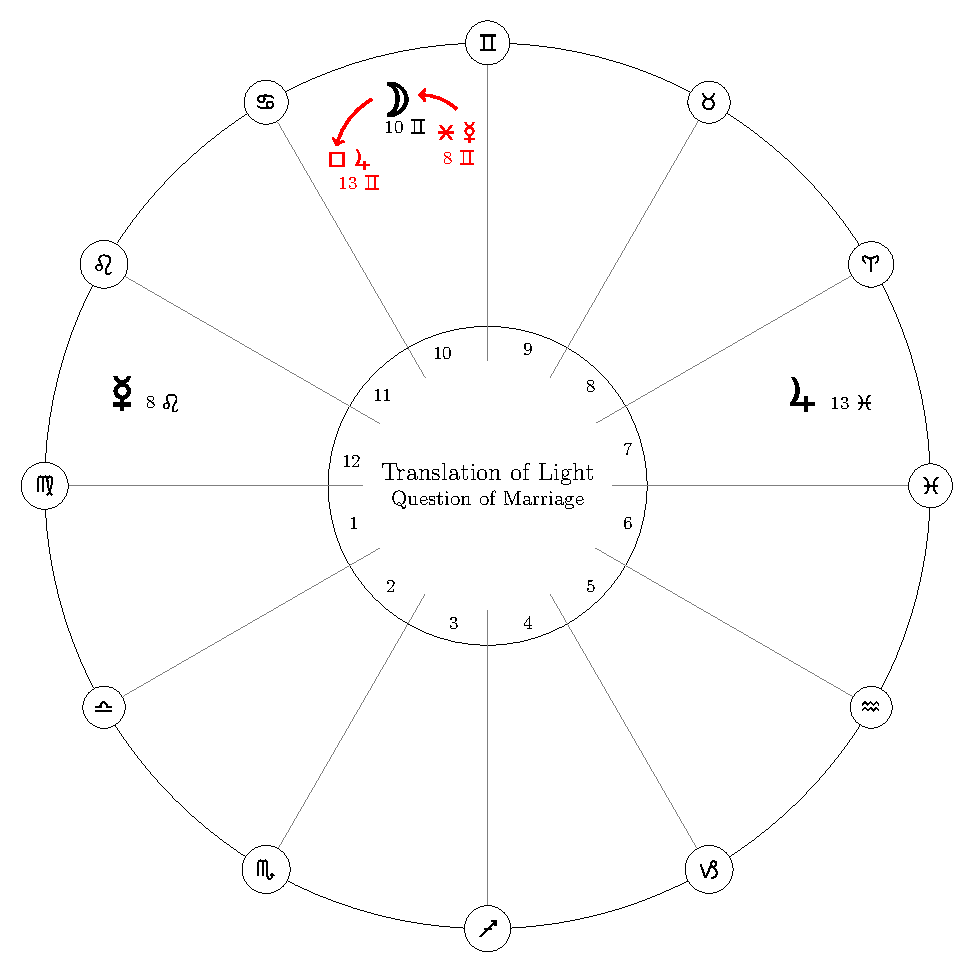
\includegraphics[width=0.9\textwidth]{charts/60-translation}} \\
\end{center}
\end{columns}
\footnotetext[1]{Ibn Ezra "conferring of nature" p121}
\end{frame}
% -------------------------------------------------------
\subsection{6. Conjunction (Collection) of Light}
\begin{frame}[t]{6. Conjunction (Collection) of LIght}
\begin{description}[style=nextline]
\item[6. Collection of Light] (\textsl{algemee}) when 2 planets, not in aspect themselves, both connect to a 3rd, heavier planet, that planet is said to collect their light

\begin{columns}[T, onlytextwidth]
\column{0.5\textwidth}
\textbf{Example:} A question about whether a king would acquire a kingdom \\
\ul
\Venus\ (L1) and \Moon\ (L10) are averse \\
\Jupiter\ is in the 10th, the house of the kingdom \\
both \Venus\ and the \Moon\ are joined to \Jupiter \\
\vspace{0.25cm}
\textsl{"This signified the acquisition of the kingdom through the hands of some judge or bishop or the hands of some chosen man to whom both planets freely gave their assent."} (p15). \\
\vspace{0.25cm}
\textbf{Note:} Another instance of a dignified benefic in the quesited house perfecting the matter without regard to reception.
\column{0.5\textwidth}
\vspace{-0.5cm}
\begin{center}
{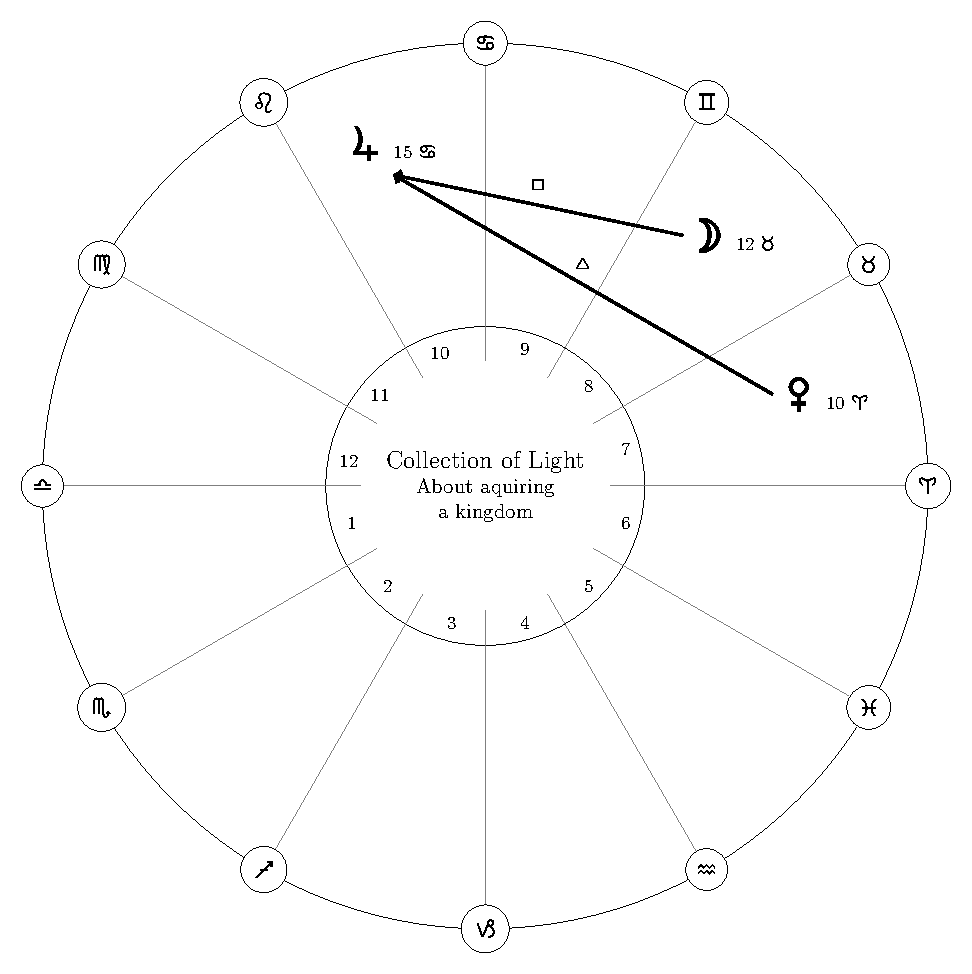
\includegraphics[width=0.9\textwidth]{charts/61-collection}} \\
\end{center}
\end{columns}
\end{description}
\end{frame}
% ------------------------------------------------
\subsection{7 Prohibition}
\begin{frame}[t]{7 Prohibition ("cutting", "intervention", "nullification")}
Prohibition (\textsl{almane}) is found in 3 modes:\footnotemark[1]  \\
\begin{columns}[T, onlytextwidth]
\column{0.5\textwidth}
\vspace{0.25cm}
\textbf{(i) Abscission ("cutting") of Light} \\
occurs when the significators are conjoining but between them is a 3rd planet who the 1st significator conjoins before it can connect with the 2nd significator. \\

\vspace{0.25cm}
\textbf{Example:} a question of marriage \\
\ul
\Mercury\ (L1) conjoins \Square\ \Mars\ before it conjoins \Trine\ \Jupiter (L7) \\
so \Mars's cuts off \Mercury's light from \Jupiter, prohibiting the marriage. \\

\vspace{0.15cm}
And Sahl says \textsl{"the destruction of this thing would be from the description of the dowry"} as \Mars\ is in the 8th house (the bride-to-be's property).

	
\column{0.5\textwidth}
\vspace{-0.5cm}
\begin{center}
{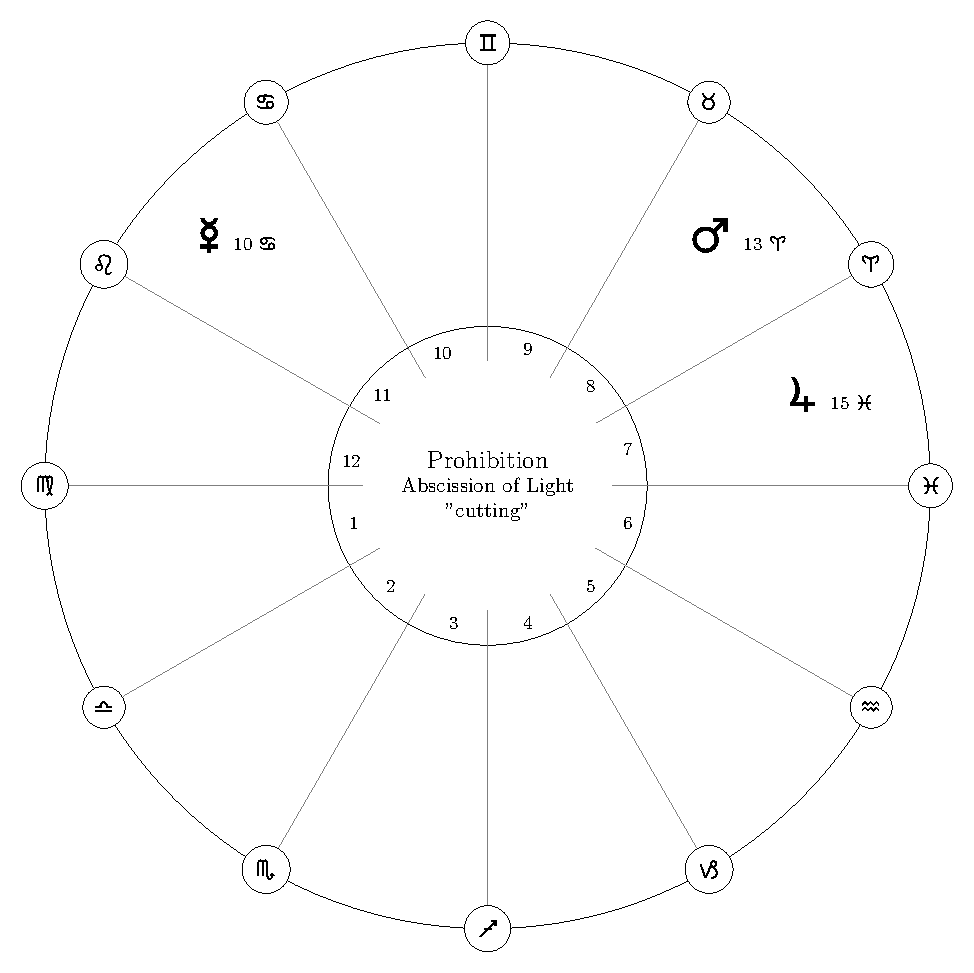
\includegraphics[width=0.9\textwidth]{charts/62-abscission}} \\
\end{center}
\end{columns}
\footnotetext[2]{Dykes calls the 3 modes  "cutting", "intervention", and "nullification" (p56-7)}
\end{frame}
% --------------------------------------------------
\begin{frame}[t]{7. Prohibition: "intervention"}
\begin{columns}[T, onlytextwidth]
\column{0.5\textwidth}
\vspace{0.5cm}
\textbf{(ii) "intervention"} occurs when 2 significators are in the same sign and a 3rd planet, between them, conjuncts the heavier, 2nd significator before the 1st significator can reach it \\

\vspace{0.25cm}
\textbf{Example:} a question of marriage \\
\ul
\Moon\ is L1 and significator of the querent \\
\Saturn\ is L7 and significator of the marriage \\

\vspace{0.25cm}
\Mars\ is between the \Moon\ and \Saturn\ and already conjoined with \Saturn\ (being only 2° from it), effectively intervening between the \Moon\ and \Saturn\ and so prohibiting the  marriage
	
\column{0.5\textwidth}
\begin{center}
{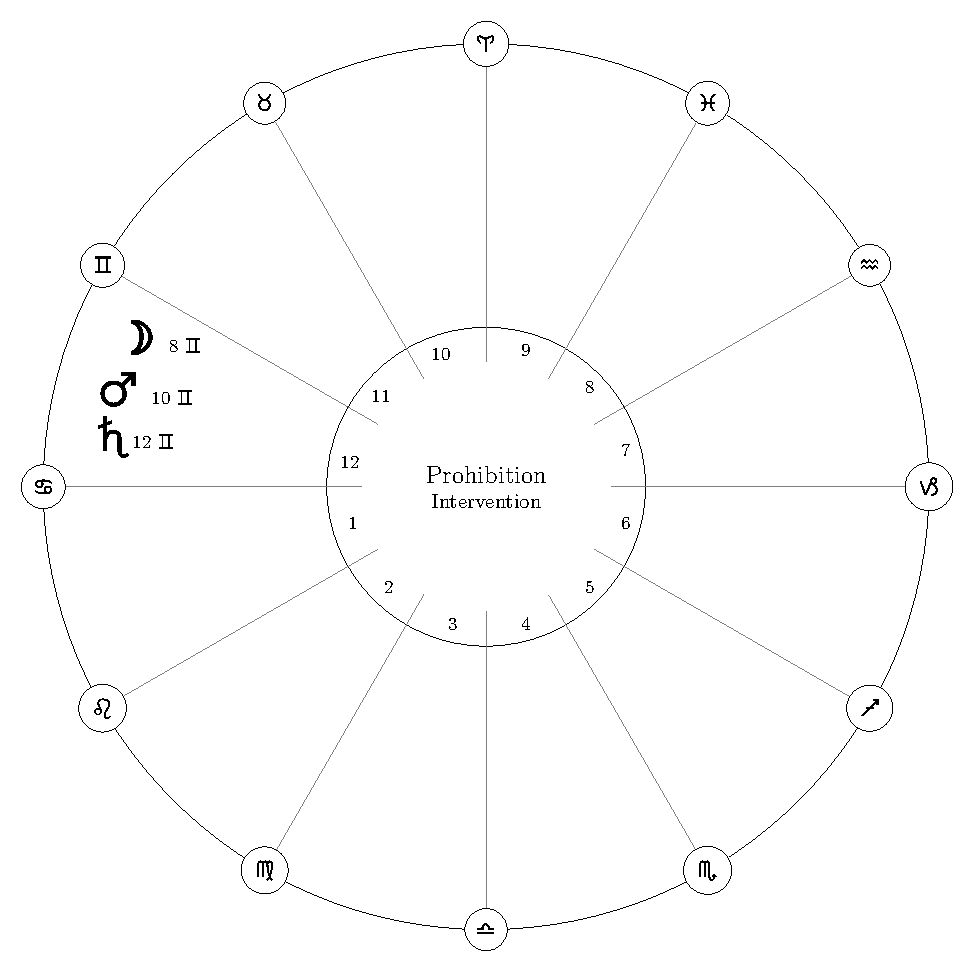
\includegraphics[width=0.9\textwidth]{charts/63-intervention}} \\
\end{center}
\end{columns}
\end{frame}
% -------------------------------------------------
\begin{frame}[t]{7. Prohibition: "nullification"}
\begin{columns}[T, onlytextwidth]
\column{0.5\textwidth}
\vspace{0.5cm}
\textbf{(iii) "nullification"} when 2 significators are in the same sign and a 3rd, lighter planet, passes the 1st significator to complete an aspect to the 2nd significator, that joining is nullified by the conjunction as \textsl{"an aspect does not destroy a conjunction, but a conjunction does destroy an aspect"} [JH p17]

\vspace{0.25cm}
\textbf{Example:} a question of marriage \\
\ul
\Moon\ is L1 and significator of the querent \\
\Saturn\ is L7 and signifcator of the marriage \\
\Mars\ is seen to be \Conjunction\ \Saturn\ (event though its fairly wide) and so \textsl{"consequently it was cutting off the aspect between the \Moon\ and \Saturn"}, prohibiting their joining and hence the marriage.

\column{0.5\textwidth}
\begin{center}
{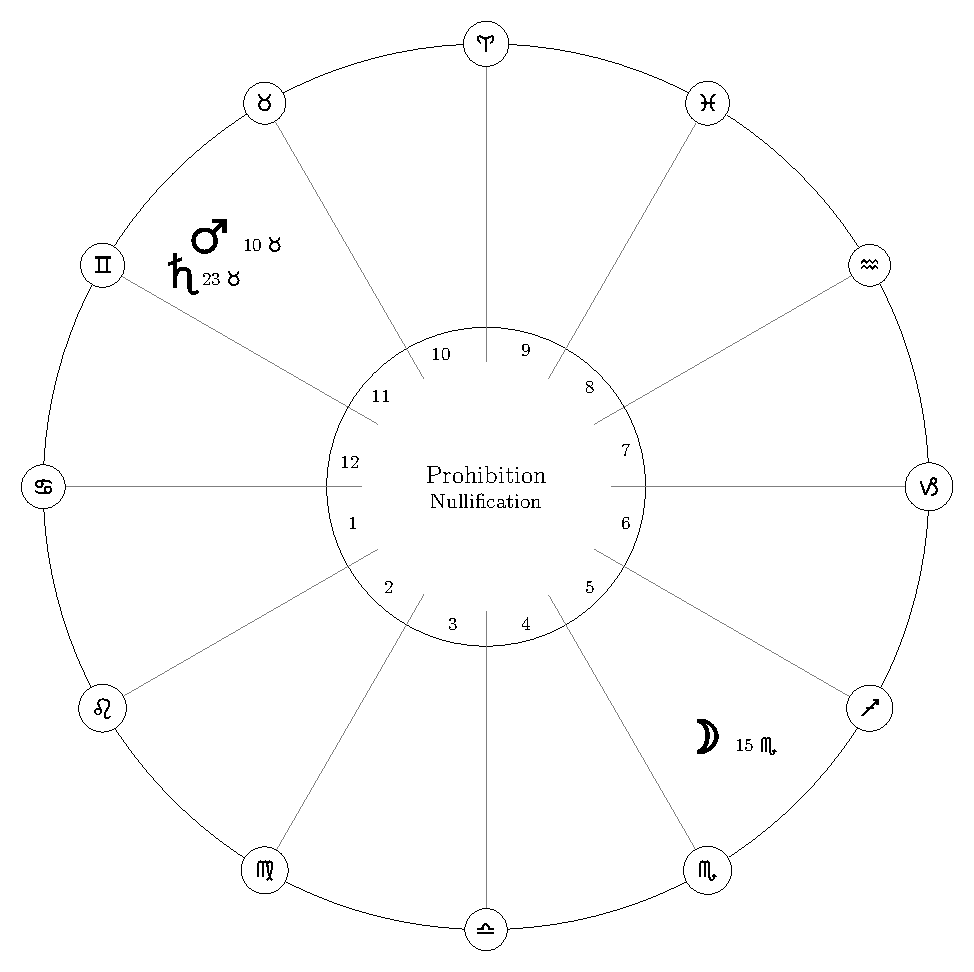
\includegraphics[width=0.9\textwidth]{charts/64-nullification}} \\
\end{center}
\end{columns}
\end{frame}
% ------------------------------------------------------
\begin{frame}[t]{7. Prohibition: "nullification" cont'd}
\begin{columns}[T, onlytextwidth]
\column{0.5\textwidth}
Another example, when two planets are joined in one sign (\Moon\ and \Mars\ here) and the lighter planet (\Moon) joins a third planet (\Venus) and commits its disposition (the two are in mutual reception), before it completes its \Conjunction\, the judgment is from the planet that is in the same sign because \textsl{"conjunction of this sort is, as we have said, stronger than an aspect."} \\

\vspace{0.25cm}
Sahl also says that \textsl{"when one planet is joined to another, but before it connects to it, it is joined to a third; and when it has been joined to that one, the conjunction itself is destroyed"} the implication being that while an aspect cannot destroy a conjunction, another conjunction can.

\column{0.5\textwidth}
\begin{center}
{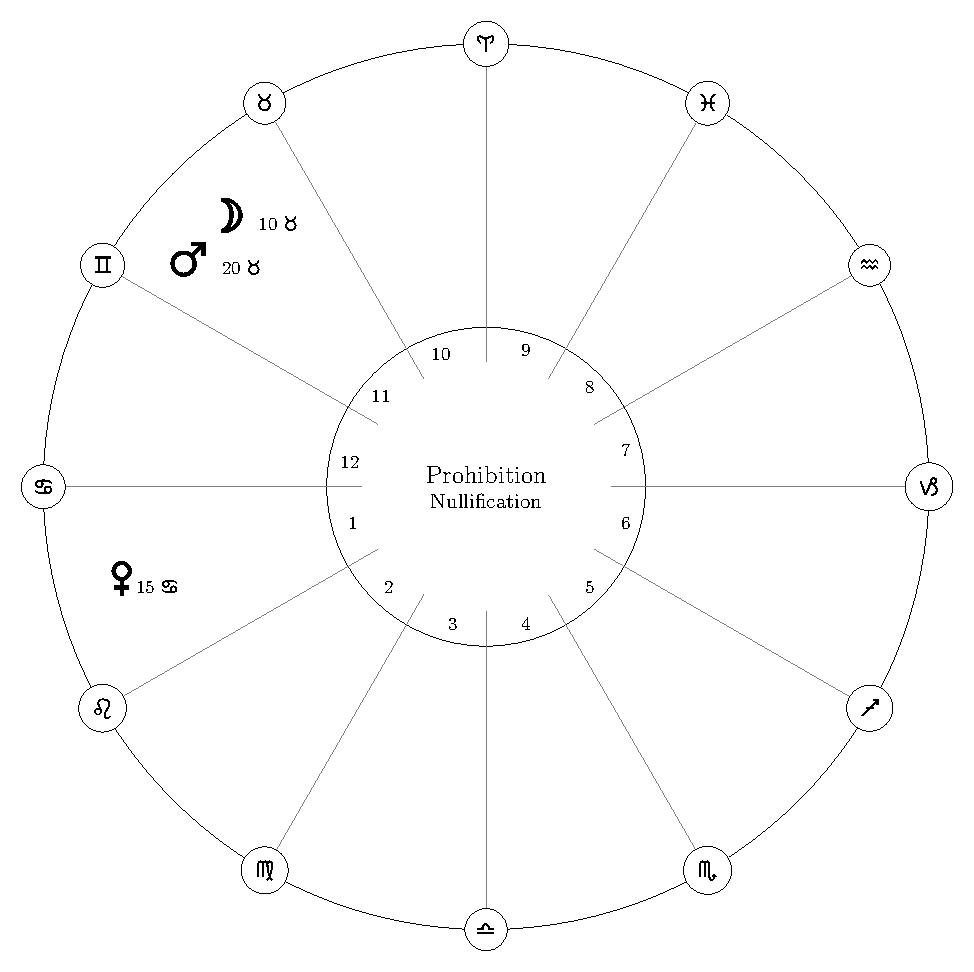
\includegraphics[width=0.9\textwidth]{charts/64a-nullification}} \\
\end{center}
\end{columns}
\end{frame}
% --------------------------------------------
\subsection{8 Reception}
\begin{frame}[t]{8. Reception}
\small
\begin{columns}[T, onlytextwidth]
\column{0.5\textwidth}
\textsl{(alchobol)} Reception occurs when a planet joins another from that planet's domicile or exaltation (perfect reception) or from two of the other planet's minor dignities (triplicity, term, face). \\

\vspace{0.25cm}
\textbf{Example:} \\
\ul
\Moon\ in \Aries\ in \Trine\ to \Mars\ in \Sagittarius \\

\vspace{0.25cm}
\Mars\ will receive the \Moon\ because she occupies his (\Mars) domicile. Similarly, if she was joined to the \Sun, as \Aries\ is his exaltation; or if she was in \Taurus\ and joined to \Venus, or in \Gemini\ and joined to \Mercury; in each case she would be received as she would occupy the domicile or exaltation of the planet she was conjoining. \\

\vspace{0.25cm}
And if the \Moon\ was void of course but on moving into the next sign she was joined to the domicile or exaltation ruler of the first sign, she will be received but if she first joins another planet in her new sign, she will be impeded [JH p19]


\column{0.5\textwidth}
\begin{center}
{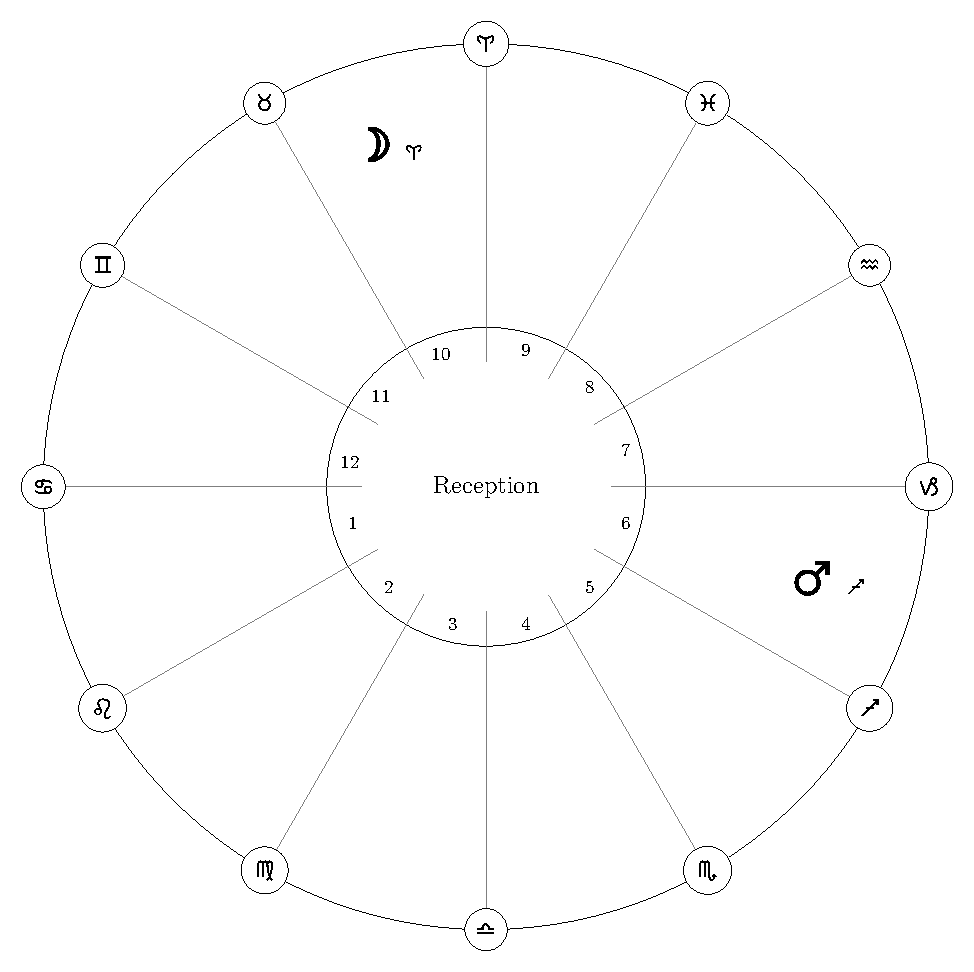
\includegraphics[width=0.9\textwidth]{charts/65-reception}} \\
\end{center}
\end{columns}
\end{frame}
% ---------------------------------
\subsection{9 Not Received}
\begin{frame}[t]{9. Not Received}
\footnotesize
\begin{columns}[T, onlytextwidth]
\column{0.5\textwidth}
\textsl{(gattalchobol)} There can be no reception between two planets (A $\Rightarrow$ B) if: \\
\vspace{0.25cm}
(i) A is in the sign of B's Fall (\Moon\ \Square\ \Saturn) \\
(ii) A is in its Fall and B is peregrine there (\Venus\ \Sextile\ \Jupiter) \\
(iii) B is peregrine in the sign A occupies (\Jupiter\ \Trine\ \Saturn)\\
(iv) B is in the sign of A's Fall (\Mercury\ \Square\ \Mars) \\
(v) B is in the sign of its own Fall \\
\hspace{1em}i.e. \Moon\ in \Gemini\ \Trine\ \Sun\ in \Libra\ (not shown) \\
\vspace{0.25cm}
According to Sahl, a planet with no \textsl{testimony} (dignity) in a place cannot recognize the planet that is applying to it and so cannot receive it. \\

And he says A in B's fall \textsl{"will be like someone who comes to him [B] from the house of his enemies--it does not receive it nor esteem it."} (i) \\

And a planet in its own Fall conjoined to a planet with no dignity in that same sign will see the other planet \textsl{"for nothing, as if an unknown garment should be given to anyone asking"}. (ii)\\

And a planet joined to another in its own Fall \textsl{"makes him descend, and it diminishes what will come to him"}. (v)

\column{0.5\textwidth}
\begin{center}
{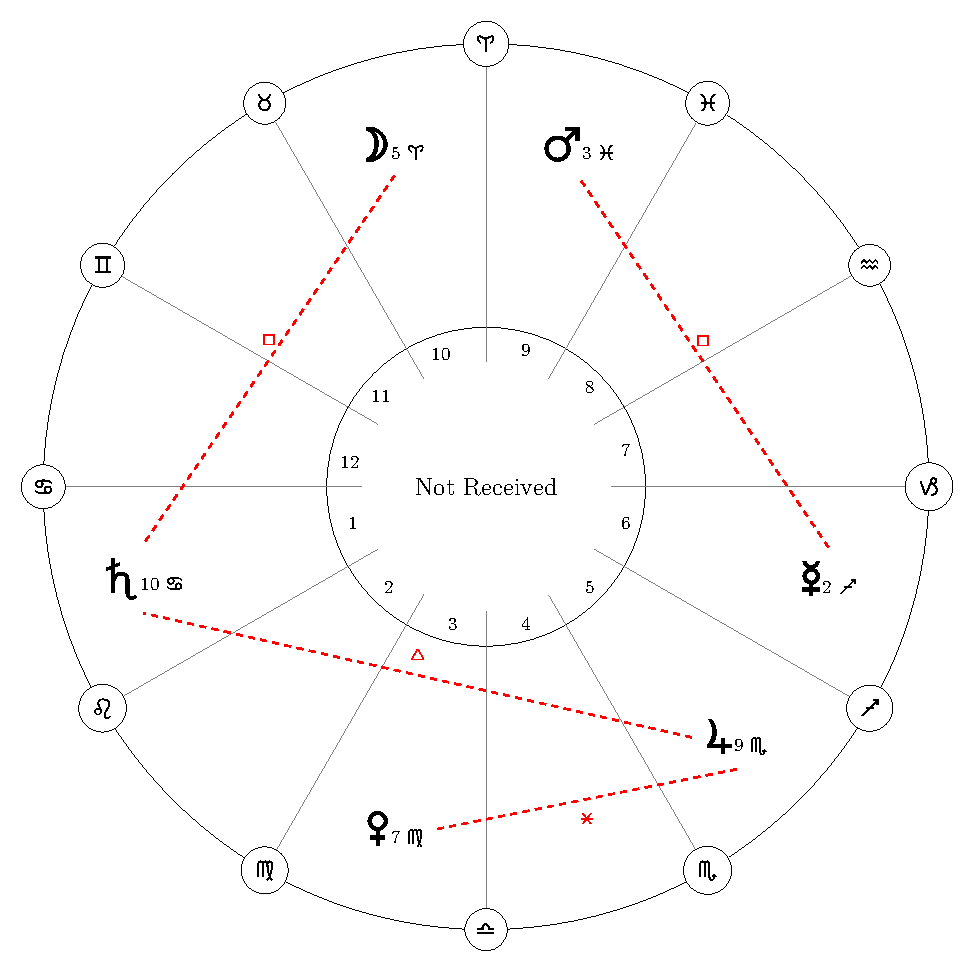
\includegraphics[width=0.9\textwidth]{charts/66-not-received}} \\
\end{center}
\end{columns}
\end{frame}
% ---------------------------------------
\subsection{10-13 Void of Course (VOC), Return, Giving Virtue}
\begin{frame}[t]{10-13 Void of Course (VOC), Return}
\begin{description}[style=nextline]
\item[10. Void of Course] \textsl{(halaaceir)} void of course occurs when a planet is not joined to (in the light of) any other planet. \textbf{Note:} this is not the same as the modern VOC  which occurs when a planet forms no aspect before leaving a sign.

\item[11. Return] \textsl{(atrad)} Return occurs when a planet is retrograde or USB. In such situations the planet will return whatever it receives, destroying the matter. The same also occurs if both planets are cadent i.e. \Moon\ in the 6th applying to \Mars\ in the 12th which \textsl{"denotes destruction of the beginning of the question and [also] its end."} And if A is angular and only B is cadent, it signifies the beginning of a matter that will not have an end.

\item[12-13. Giving Virtue and Nature] \textsl{(defaalchota)} a planet in its own domicile or exaltation is joined to another planet i.e. \Moon\ in \Cancer\ or \Taurus\ joined to \Jupiter\ or any other planet \textsl{"gives its virtue"} (nature) and commits its disposition. When she is not in \Taurus\ or \Cancer\ she just gives her dispostion.\footnotemark[1]
\end{description}
\footnotetext[1]{Here I think \textsl{disposition} refers to a planet's significations while \textsl{virtue} refers to its authority and power.}
\end{frame}



